%%
% Plantilla de Presentación
% Modificación de una plantilla de Latex de LaTeXTemplates para adaptarla 
% al castellano y a las necesidades de escribir informática y matemáticas.
%
% Editada por: Mario Román
%
% License:
% CC BY-NC-SA 3.0 (http://creativecommons.org/licenses/by-nc-sa/3.0/)
%%

%%%%%%%%%%%%%%%%%%%%%
% Beamer Presentation
% LaTeX Template
% Version 1.0 (10/11/12)
%
% This template has been downloaded from:
% http://www.LaTeXTemplates.com
%
% License:
% CC BY-NC-SA 3.0 (http://creativecommons.org/licenses/by-nc-sa/3.0/)
%
%%%%%%%%%%%%%%%%%%%%%

%----------------------------------------------------------------------------------------
%	PAQUETES Y CONFIGURACIÓN DEL DOCUMENTO
%----------------------------------------------------------------------------------------

\documentclass[12pt, aspectratio=169]{beamer} % Beamer
\usepackage[spanish]{babel} % Traducciones
\usepackage[utf8]{inputenc} % Uso de caracteres UTF-8
\usepackage[T1]{fontenc} % Permite copiar código y evita errores
\uselanguage{Spanish} % Traducciones beamer
\languagepath{Spanish} % (tex.stackexchange.com/questions/168208)
\usepackage{pgfpages} % Beamer User Guide sections 19.6 and 22
\usepackage[absolute,overlay]{textpos} % Especifica posición del texto.

%% Temas %%
% Tema y tema de color
\usetheme{Dresden}
\usecolortheme{dolphin}

% Fuentes de tamaño arbitrario
\usepackage{lmodern}

% Gráficos
\usepackage{graphicx} % Allows including images
\usepackage{booktabs} % Allows the use of \toprule, \midrule and \bottomrule in tables

%----------------------------------------------------------------------------------------
%	TÍTULO
%----------------------------------------------------------------------------------------

%% Título y otros %%
\title[Análisis de TC, WF y GF]{Análisis comparativo de los servidores de aplicaciones
Apache Tomcat, WildFly y GlassFish} % The short title appears at the bottom of every slide, the full title is only on the title page

% Se supone que es anónima
\author[Óscar Bermúdez]{
	Óscar Bermúdez\\	
	\href{http://www.github.com/oxcar103}{@oxcar103}
} % Your name

\institute[UGR] % Your institution as it will appear on the bottom of every slide, may be shorthand to save space
{
  Universidad de Granada \\ % Your institution for the title page
}
\date{\today} % Date, can be changed to a custom date

\begin{document}

% Diapositiva de título.
\begin{frame}
	\titlepage % Print the title page as the first slide
\end{frame}


%----------------------------------------------------------------------------------------
%	PRESENTACIÓN
%----------------------------------------------------------------------------------------

%------------------------------------------------

\section{Introducción}
	\begin{frame}
		Para el desarrollo de servidores webs, se requieren del manejo de instrucciones de administración
		de servidores como pueden ser:
		
		\begin{itemize}
			\item \uncover<2->{Control de seguridad}
			
			\only<3>{\begin{figure}
				
\includegraphics[width=5cm]{Thief.jpg}
			\end{figure}}

			\item \uncover<4->{Gestión de concurrencia}
			
			\only<5>{\begin{figure}
				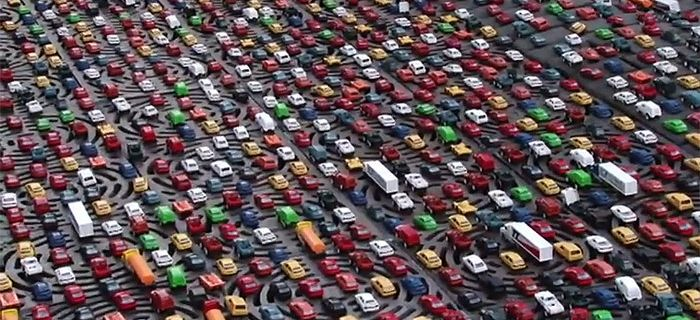
\includegraphics[width=10cm]{Atasco.jpg}
			\end{figure}}
			
			\item \uncover<6->{Manejo de peticiones de clientes}
			
			\only<7>{\begin{figure}
				
\includegraphics[width=10cm]{Burocracia.jpg}
			\end{figure}}

		\end{itemize}

		\uncover<8->{Esto provoca que el desarrollador haga un esfuerzo adicional que distrae la atención
		sobre la lógica de negocio.}
	\end{frame}

\section{Java EE}
	\begin{frame}
		Para remediar esta situación, se desarrollan plataformas de programación de desarrollo que
		se encargan de esas tareas de mantenimiento.
		
		Estas plataformas disponen de un conjunto de rutinas, protocolos y herramientas para favorecer
		el desarrollo de aplicaciones software, así como pequeños programas que se ejecutan en segundo
		plano y se encargan de la gestión del servidor y de la generación de páginas dinámicas.
		
		Hay varias plataformas desarrolladas en distintos lenguajes de programación.
		
		\pause
		
		\alert{En este caso, nos centraremos en Java Platform, Enterprise Edition o Java EE que es un plataforma
		desarrollada en Java.}
	\end{frame}

\section{Presentación de los programas}
	\subsection{Apache Tomcat}
		\begin{frame}
			\frametitle{Apache Tomcat}
			
			\begin{figure}
				
\includegraphics[width=3cm]{Tomcat_logo.jpg}
			\end{figure} 
			
			\pause
			
			Apache Tomcat(o simplemente Tomcat), es un contenedor de Servlet y JavaServer
			Pages multiplataforma implementado en Java en código abierto.
			
			Fue desarrollado inicialmente por James Duncan(que era empleado de \textit{Sun
			Microsystems}) y donado posteriormente a la \textit{Apache Software Foundation (ASF)}.
			
			A diferencia de los otros proyectos, no es un servidor de aplicaciones, por ello,
			se desarrolló Apache TomEE que lo extiende utilizando para ello las características
			propias de JavaEE.
		\end{frame}

	\subsection{WildFly}
		\begin{frame}
			\frametitle{WildFly}
			
			\begin{figure}
				
\includegraphics[width=3cm]{WildFly_logo.jpg}
			\end{figure}
			
			\pause
			
			WildFly es un servidor de aplicaciones multiplataforma implementado en Java en
			código abierto.
			
			Inicialmente, se llamó JBoss y fue desarrollado por Marc Fleury, que fue otro
			empleado de \textit{Sun Microsystem}. Más tarde, \textit{RedHat} lo compró. Y hace
			unos años, se realizó una votación pública en la que se le cambió de nombre por el
			actual.
			
		\end{frame}
	
	\subsection{GlassFish}
		\begin{frame}
			\frametitle{GlassFish}
			
			\begin{figure}
				
\includegraphics[width=3cm]{GlassFish_logo.jpg}
			\end{figure}
			
			\pause
			
			GlassFish también es un servidor de aplicaciones implementado en Java en código abierto.
			
			Como los dos anteriores, fue desarrollado inicialmente por \textit{Sun Microsystems}.
			Posteriormente, \textit{Oracle Corporation} adquirió la compañía y pasó a encargarse del
			desarrollo de este proyecto.
			
		\end{frame}

\section{Comparación}
	\begin{frame}
		\frametitle{Tomcat}
		
		Ahora queda realizar las medidas a cada servidor con los comandos \textit{ab} y \textit{sar}:
		
		\only<2>{\begin{figure}
			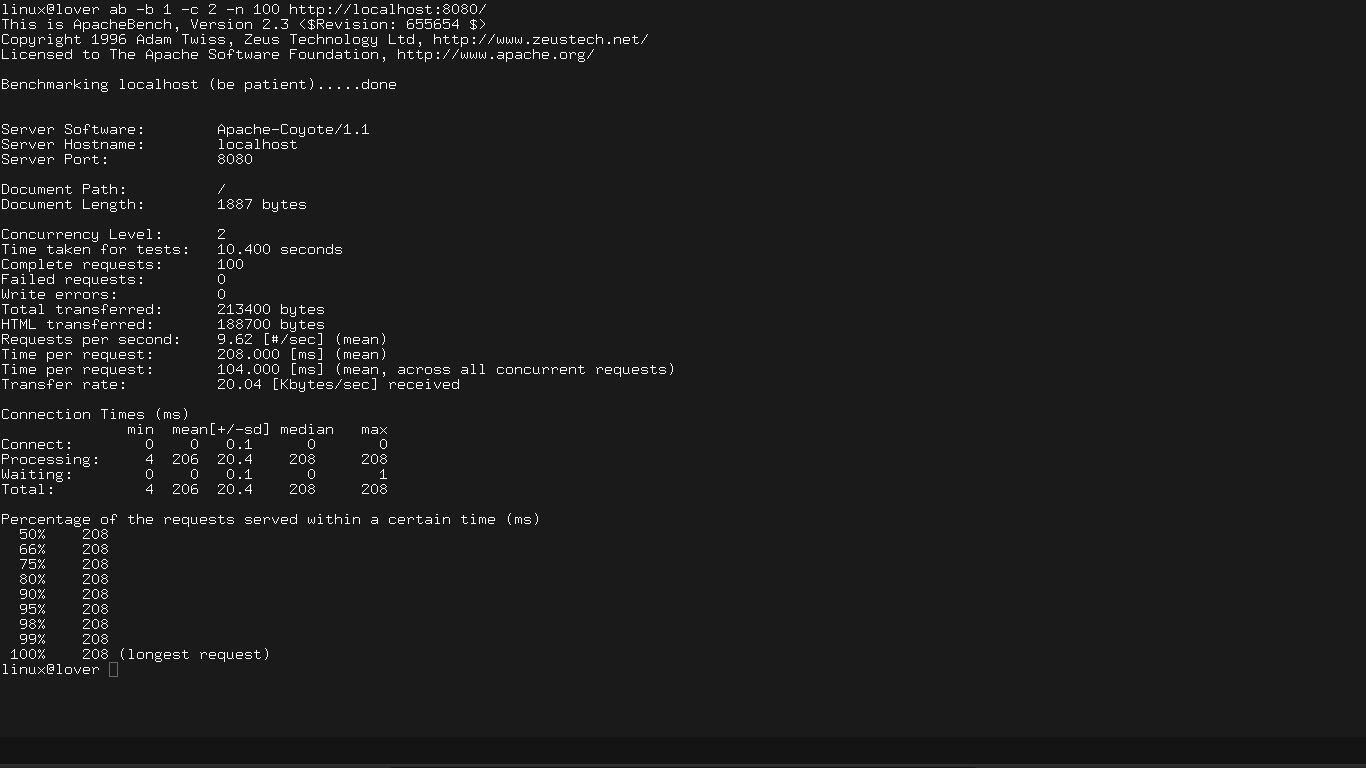
\includegraphics[width=10cm]{AB.png}
		\end{figure}}
		
		
		\only<3>{\begin{figure}
			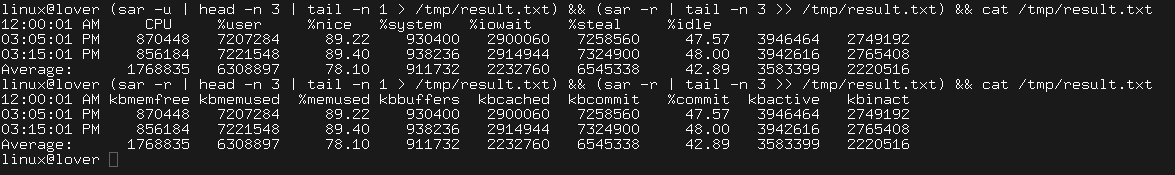
\includegraphics[width=14cm]{SAR.png}
		\end{figure}}
	\end{frame}

	\begin{frame}
		\frametitle{Fracaso...}
		
		Desgraciadamente, no he logrado instalar bien los otros dos programas...
		
		\pause
		
		\begin{figure}
			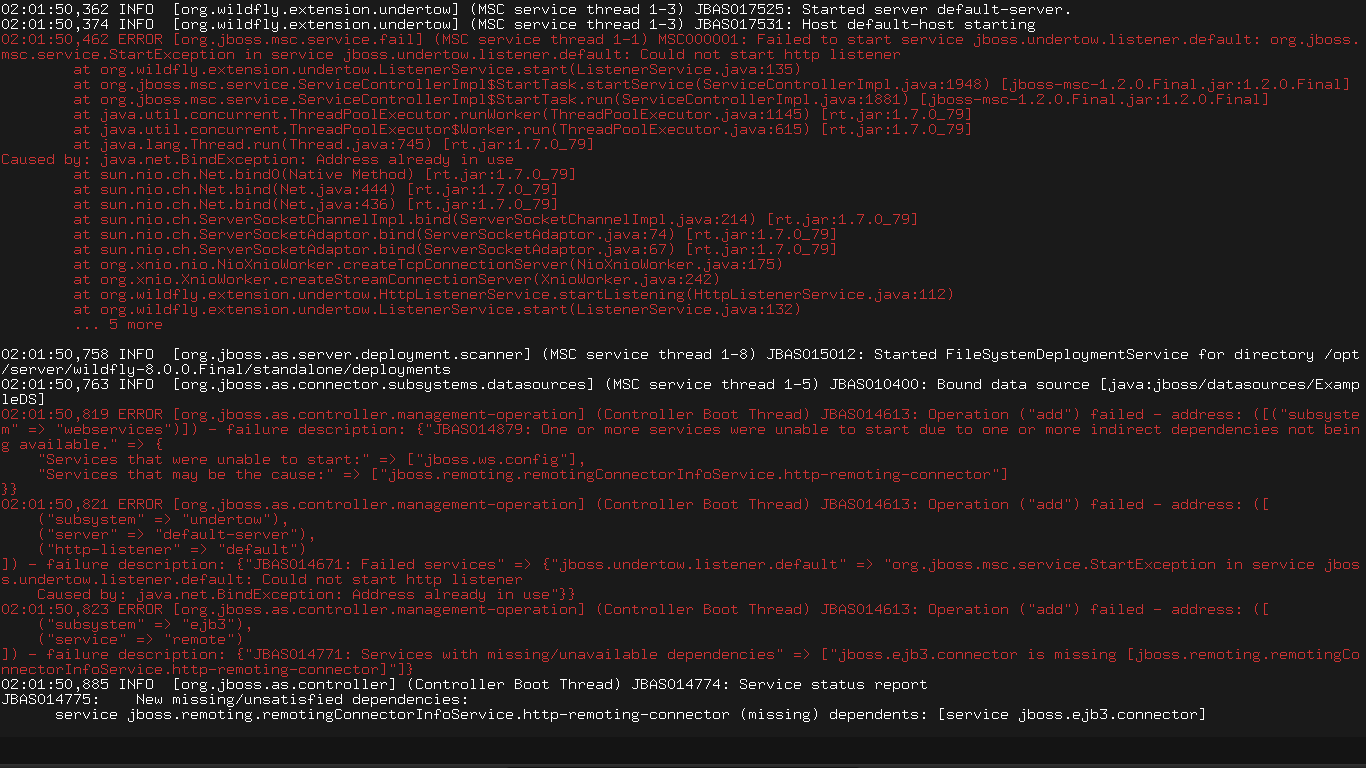
\includegraphics[width=8cm]{Fail_WF.png}
		\end{figure}
		
		\pause
		
		Así que la comparativa no ha sido posible.
		
	\end{frame}


\section{Referencias}
	% Bibliografía
	\begin{frame}
		\frametitle{Referencias}
		
		Para la realización de estas diapositivas, se han utilizado los repositorios de GitHub:
		
		\footnotesize{
		  \begin{thebibliography}{7} % Beamer does not support BibTeX so references must be inserted manually as below
		    \bibitem{Pbaeyens} Pablo Baeyens
		      \newblock Guía de uso de beamer
		      \newblock \url{https://github.com/dgiim/beamer}
		      
		    \bibitem{M42} Mario Román
		      \newblock Recopilación de plantillas de Latex.
		      \newblock \url{https://github.com/M42/plantillas}
		  \end{thebibliography}
		}
	\end{frame}

%------------------------------------------------

\begin{frame}
\Huge{\centerline{Fin.}}
\end{frame}

%----------------------------------------------------------------------------------------

\end{document}
